% Entrega 1 — ALU takum e instruções vetoriais básicas (Zvtakum)
% Compilar: latexmk -pdf entrega1.tex   (ou: make -C docs/entrega1)
\documentclass[11pt,a4paper]{article}

\usepackage[T1]{fontenc}
\usepackage[utf8]{inputenc}
\usepackage[brazilian]{babel}
\usepackage{lmodern}
\usepackage[margin=2.5cm]{geometry}
\usepackage{amsmath,amssymb}
\usepackage{booktabs}
\usepackage{tabularx}
\usepackage{listings}
\usepackage{xcolor}
\usepackage{tikz}
\usetikzlibrary{arrows.meta,positioning,fit,calc}
\usepackage{enumitem}
\usepackage{float}
\usepackage[hidelinks]{hyperref}


\lstset{
  basicstyle=\ttfamily\small,
  columns=fullflexible,
  keepspaces=true,
  frame=single,
  framesep=4pt,
  rulecolor=\color{black!30},
  extendedchars=false,
  showstringspaces=false,
}

% Estilo para os arquivos-fonte incluídos no apêndice (comentários em português, UTF-8)
\lstdefinestyle{src}{
  upquote=true,
  basicstyle=\ttfamily\footnotesize,
  keywordstyle=\color{blue!60!black}\bfseries,
  commentstyle=\color{green!40!black}\itshape,
  stringstyle=\color{red!50!black},
  numbers=left,
  numberstyle=\tiny\color{black!50},
  numbersep=6pt,
  xleftmargin=1.5em,
  breaklines=true,
  breakatwhitespace=false,
  tabsize=4,
  extendedchars=true,
  literate=
    {á}{{\'a}}1 {à}{{\`a}}1 {ã}{{\~a}}1 {â}{{\^a}}1
    {é}{{\'e}}1 {ê}{{\^e}}1 {í}{{\'i}}1 {ó}{{\'o}}1
    {õ}{{\~o}}1 {ô}{{\^o}}1 {ú}{{\'u}}1 {ç}{{\c{c}}}1
    {Á}{{\'A}}1 {É}{{\'E}}1 {Ç}{{\c{C}}}1 {º}{{\textordmasculine}}1
    {—}{{---}}1 {–}{{--}}1 {−}{{-}}1 {≥}{{$\geq$}}1 {≤}{{$\leq$}}1
    {×}{{$\times$}}1 {→}{{$\rightarrow$}}1
}
\lstdefinelanguage{Verilog2005}[]{Verilog}{
  morekeywords={localparam,generate,endgenerate,genvar,signed,integer,wire,reg},
}
\newcommand{\srcfile}[3][Verilog2005]{%
  \lstinputlisting[style=src, language=#1, caption={\texttt{\detokenize{#2}} --- #3}]{../../#2}}
% Trecho de um arquivo do repositório: \srctrecho{arquivo}{primeira}{última}{legenda}
\newcommand{\srctrecho}[4]{%
  \lstinputlisting[style=src, language=Verilog2005, firstline=#2, lastline=#3, firstnumber=#2,
    caption={\texttt{\detokenize{#1}}, linhas #2--#3: #4}]{../../#1}}
\renewcommand{\lstlistingname}{Código}
\renewcommand{\lstlistlistingname}{Lista de códigos}

\newcommand{\code}[1]{\texttt{#1}}

\title{\textbf{Entrega 1 --- ALU Takum e Instruções Vetoriais Básicas}\\[4pt]
\large Projeto Integrador AOC 2026/02 --- Formato Takum na Extensão Vetorial RISC-V}
\author{%
  Heloisa Silva Rosa \and Samantha Kelly de Souza Sena \and Vitor Hugo Lacerda Lana\\[4pt]
  \small Arquitetura e Organização de Computadores --- DELT/UFMG}
\date{Outubro de 2026}

\begin{document}
\maketitle

\noindent\textbf{Resumo.} Relatório parcial das semanas 3--4. Implementamos em Verilog o decodificador,
o codificador e a ALU (soma, subtração e multiplicação) do formato \emph{takum} linear para T8, T16 e T32,
além de uma unidade vetorial com as instruções \code{vtadd.vv}, \code{vtsub.vv} e \code{vtmul.vv}.
Todos os testes passam. Este documento não é o artigo final.

%======================================================================
\section{O que foi feito}

\begin{table}[H]
\centering
\begin{tabularx}{\linewidth}{Xl}
\toprule
Item & Situação \\
\midrule
Decodificador e codificador takum (T8, T16, T32) & pronto, testado \\
ALU: soma, subtração e multiplicação & pronta, testada \\
Unidade vetorial \code{vtadd.vv}, \code{vtsub.vv}, \code{vtmul.vv} & pronta, testada \\
\code{vtdot.vv}, \code{vncvt.t.t}, integração no modelo RVV & Fase 2 \\
Benchmarks de álgebra linear esparsa e erro relativo & Fase 3 \\
\bottomrule
\end{tabularx}
\end{table}

O código está no repositório: RTL em \code{rtl/}, testes em \code{tb/}. Para rodar: \code{make test}.

%======================================================================
\section{Formato takum}

Usamos o takum linear de Hunhold~\cite{hunhold2024takum}. Uma palavra de $n$ bits tem os campos
$S$ (sinal), $D$ (direção), $R$ (regime, 3 bits), $C$ (característica, $r$ bits) e $F$ (fração):
\[
r = \begin{cases} R & D=1\\ 7-R & D=0 \end{cases}
\qquad
c = \begin{cases} 2^r - 1 + C & D=1\\ -2^{r+1} + 1 + C & D=0 \end{cases}
\qquad
x = (1 + f)\cdot 2^{c} \;\; (x > 0).
\]
Negativos são o complemento de dois da palavra. $00\cdots0$ é zero e $10\cdots0$ é NaR.
O que importa para o hardware: os campos $S$, $D$, $R$, $C$ cabem sempre nos 12 primeiros bits,
para qualquer $n$.

%======================================================================
\section{Arquitetura}

Toda operação passa por três blocos combinacionais (Figura~\ref{fig:datapath}):

\begin{figure}[H]
\centering
\begin{tikzpicture}[
  blk/.style={draw, rounded corners=2pt, minimum height=9mm, align=center, font=\small},
  arr/.style={-{Latex[length=2mm]}}]
  \node[blk, minimum width=24mm] (da) at (0, 0.8) {decodificador};
  \node[blk, minimum width=24mm] (db) at (0,-0.8) {decodificador};
  \node[blk, minimum width=24mm, minimum height=25mm] (core) at (4,0) {núcleo\\ add / sub / mul};
  \node[blk, minimum width=24mm] (enc) at (8,0) {codificador\\ \scriptsize arredonda e satura};
  \node (a) at (-2.2, 0.8) {$a$};
  \node (b) at (-2.2,-0.8) {$b$};
  \node (y) at (10.2,0) {$y$};
  \draw[arr] (a) -- (da);  \draw[arr] (b) -- (db);
  \draw[arr] (da.east) -- (core.west |- da.east);
  \draw[arr] (db.east) -- (core.west |- db.east);
  \draw[arr] (core) -- (enc);  \draw[arr] (enc) -- (y);
\end{tikzpicture}
\caption{Caminho de dados da \code{takum\_alu}.}
\label{fig:datapath}
\end{figure}

\begin{itemize}
  \item \textbf{Decodificador} (\code{takum\_decoder}): converte a palavra em sinal, expoente (9 bits)
        e fração. Nega a palavra se for negativa e lê os 12 bits de cima com um bloco fixo
        (\code{takum\_hdr\_dec}), o mesmo para T8, T16 e T32.
  \item \textbf{Núcleo} (\code{takum\_alu}):
        \emph{multiplicação} soma os expoentes e multiplica os significandos;
        \emph{soma/subtração} alinha o menor operando, soma ou subtrai e normaliza.
        A subtração é $a + (-b)$. Os bits descartados viram \emph{guard}, \emph{round} e \emph{sticky}.
  \item \textbf{Codificador} (\code{takum\_encoder}): monta a palavra de volta, arredonda para o
        mais próximo (empate para o par) e satura: um resultado não nulo nunca vira 0 nem NaR.
\end{itemize}

O arredondamento é feito direto na palavra, porque o takum é monótono: somar 1 ao padrão de bits
leva ao próximo valor representável.

\srctrecho{rtl/takum_encoder.v}{57}{62}{arredondamento}

\paragraph{Casos especiais.} NaR em qualquer operando dá NaR; $x - x = +0$; $0 \times x = 0$.

\paragraph{Unidade vetorial} (\code{takum\_vec\_alu}). Calcula \code{vd[i] = vs2[i] op vs1[i]} para
\code{i < vl} e mantém \code{vd[i]} nos demais elementos. A largura do elemento (\code{sew} = 8, 16 ou 32)
escolhe qual fileira de ALUs vai para a saída. Máscaras e CSRs ficam para a Fase~2.

%======================================================================
\section{Verificação}

A ALU é comparada com um oráculo em Python (\code{tb/takum\_oracle.py}) que calcula o resultado exato
com frações e não compartilha código com o RTL.

\begin{table}[H]
\centering
\caption{Resultado de \code{make test}.}
\begin{tabular}{lrc}
\toprule
Teste & Casos & Resultado \\
\midrule
Decodificador (T8/T16 completos, T32 amostrado) & 265\,800 & PASS \\
Ida e volta \code{encoder(decoder(t)) == t} & 265\,792 & PASS \\
Codificador (arredondamento, empates, saturação) & 323\,816 & PASS \\
ALU T8 (todos os pares, 3 operações) & 196\,608 & PASS \\
ALU T16 / T32 (bordas e aleatórios) & 109\,923 cada & PASS \\
Unidade vetorial SEW 8/16/32 & 5\,000 cada & PASS \\
\bottomrule
\end{tabular}
\end{table}

Para conferir que os testes pegam erros, inserimos cinco defeitos de propósito na ALU
(por exemplo, esquecer o \emph{sticky} ou não normalizar o produto). Todos foram detectados.

A Figura~\ref{fig:ondas} mostra o codificador arredondando, gerada com \code{make waves}.

\begin{figure}[H]
\centering
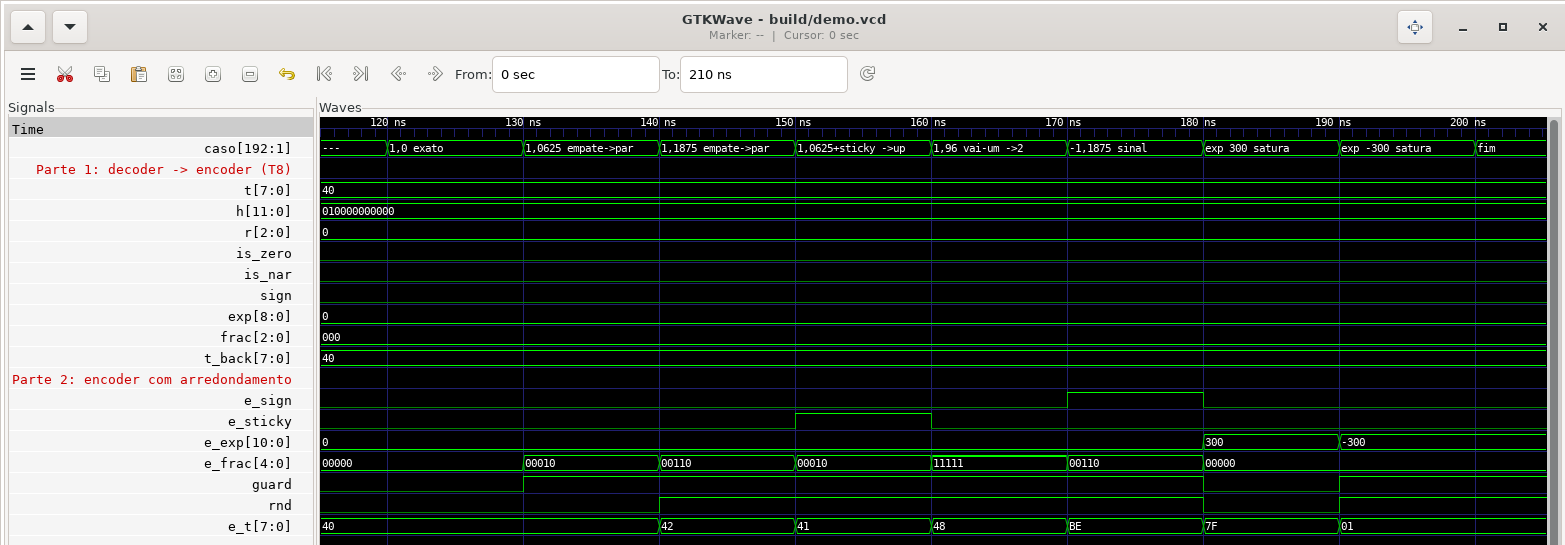
\includegraphics[width=\linewidth]{../img/ondas-parte2-encoder.png}
\caption{Codificador T8 no GTKWave: \code{rnd} indica quando a palavra é incrementada. Em 1,0625 o empate
fica no par (\code{40}); em 1,1875 sobe (\code{42}); com expoente $\pm 300$ satura (\code{7F}, \code{01}).}
\label{fig:ondas}
\end{figure}

%======================================================================
\section{Custo de hardware}

Síntese genérica com Yosys (\code{make synth}). Serve para comparar tamanhos, não como área real.

\begin{table}[H]
\centering
\begin{tabular}{lccc}
\toprule
LUT6 & T8 & T16 & T32 \\
\midrule
\code{takum\_decoder} & 46  & 89  & 164 \\
\code{takum\_encoder} & 69  & 112 & 209 \\
\code{takum\_alu}     & 327 & 912 & 2\,838 \\
\bottomrule
\end{tabular}
\end{table}

O bloco do cabeçalho custa 41 LUT6 em qualquer tamanho. Em T32 o multiplicador domina a ALU.

%======================================================================
\section{Próximos passos}

\begin{itemize}[nosep]
  \item Fase 2: \code{vtdot.vv}, \code{vncvt.t.t} e integração ao modelo RVV.
  \item Fase 3: multiplicação matriz esparsa $\times$ vetor e erro relativo contra IEEE~754 e Float128.
  \item Comparar a área com uma ALU IEEE~754 equivalente.
\end{itemize}

%======================================================================
\begin{thebibliography}{9}
\bibitem{hunhold2024takum}
L.~Hunhold, ``Beating posits at their own game: Takum arithmetic,'' in \emph{CoNGA 2024}, LNCS 14666,
Springer, 2024. arXiv:2404.18603.

\bibitem{hunhold2025avx}
L.~Hunhold, ``Streamlining SIMD ISA extensions with takum arithmetic: A case study on Intel AVX10.2,''
\emph{MOCAST}, 2025. arXiv:2503.14067.
\end{thebibliography}

%======================================================================
\clearpage
\appendix
\section{Código RTL}

\srcfile{rtl/takum_hdr_dec.v}{cabeçalho de 12 bits}
\srcfile{rtl/takum_decoder.v}{decodificador}
\srcfile{rtl/takum_encoder.v}{codificador}
\srcfile{rtl/takum_alu.v}{ALU}
\srcfile{rtl/takum_vec_alu.v}{unidade vetorial}

\end{document}
